%
% Niniejszy plik stanowi przykład formatowania pracy magisterskiej na
% Wydziale MIM UW.  Szkielet użytych poleceń można wykorzystywać do
% woli, np. formatujac wlasna prace.
%
% Zawartosc merytoryczna stanowi oryginalnosiagniecie
% naukowosciowe Marcina Wolinskiego.  Wszelkie prawa zastrzeżone.
%
% Copyright (c) 2001 by Marcin Woliński <M.Wolinski@gust.org.pl>
% Poprawki spowodowane zmianami przepisów - Marcin Szczuka, 1.10.2004
% Poprawki spowodowane zmianami przepisow i ujednolicenie 
% - Seweryn Karłowicz, 05.05.2006
% Dodanie wielu autorów i tłumaczenia na angielski - Kuba Pochrybniak, 29.11.2016

% dodaj opcję [licencjacka] dla pracy licencjackiej
% dodaj opcję [en] dla wersji angielskiej (mogą być obie: [licencjacka,en])
\documentclass[licencjacka]{pracamgr}


% Dane magistranta:
\autor{Michał Izworski}{360968}


% Dane magistrantów:
%\autor{Autor Zerowy}{342007}
%\autori{Autor Pierwszy}{342013}
%\autorii{Drugi Autor-Z-Rzędu}{231023}
%\autoriii{Trzeci z Autorów}{777321}
%\autoriv{Autor nr Cztery}{432145}
%\autorv{Autor nr Pięć}{342011}

\title{AlphaSoccer: gra w ,,Piłkarzyki~na~kartce'' za pomocą głębokich sieci neuronowych}


%\tytulang{An implementation of a difference blabalizer based on the theory of $\sigma$ -- $\rho$ phetors}

%kierunek: 
% - matematyka, informacyka, ...
% - Mathematics, Computer Science, ...
\kierunek{Międzykierunkowe Studia Ekonomiczno-Matematyczne}

% informatyka - nie okreslamy zakresu (opcja zakomentowana)
% matematyka - zakres moze pozostac nieokreslony,
% a jesli ma byc okreslony dla pracy mgr,
% to przyjmuje jedna z wartosci:
% {metod matematycznych w finansach}
% {metod matematycznych w ubezpieczeniach}
% {matematyki stosowanej}
% {nauczania matematyki}
% Dla pracy licencjackiej mamy natomiast
% mozliwosc wpisania takiej wartosci zakresu:
% {Jednoczesnych Studiow Ekonomiczno--Matematycznych}

% \zakres{Tu wpisac, jesli trzeba, jedna z opcji podanych wyzej}

% Praca wykonana pod kierunkiem:
% (podać tytuł/stopień imię i nazwisko opiekuna
% Instytut
% ew. Wydział ew. Uczelnia (jeżeli nie MIM UW))
\opiekun{prof. dr hab. Andrzej Skowron\\
  Wydział Matematyki, Informatyki i Mechaniki\\
  }

% miesiąc i~rok:
\date{Czerwiec 2018}

%Podać dziedzinę wg klasyfikacji Socrates-Erasmus:
\dziedzina{ 
%11.0 Matematyka, Informatyka:\\ 
%11.1 Matematyka\\ 
%11.2 Statystyka\\ 
%11.3 Informatyka\\ 
11.4 Sztuczna inteligencja\\ 
%11.5 Nauki aktuarialne\\
%11.9 Inne nauki matematyczne i informatyczne
}

%Klasyfikacja tematyczna wedlug AMS (matematyka) lub ACM (informatyka)
\klasyfikacja{Computing methodologies\\
	Machine learning\\
 	Learning paradigms\\
	Reinforcement learning\\
	Sequential decision making}

% Słowa kluczowe:
\keywords{machine learning, reinforcement learning, deep learning, actor-critic methods, monte carlo tree search}

% Tu jest dobre miejsce na Twoje własne makra i~środowiska:
\newtheorem{defi}{Definicja}[section]
\usepackage{wrapfig}
\usepackage{graphicx}
\graphicspath{ {img/} }
\usepackage{amsfonts}
\usepackage{amsmath}

% koniec definicji

\begin{document}

\maketitle

%tu idzie streszczenie na strone poczatkowa
\begin{abstract}
  TO DO
\end{abstract}

\tableofcontents
%\listoffigures
%\listoftables

\chapter{Wprowadzenie}\label{r:intro}

%Sztuczna inteligencja cieszy się ogromnym wzrostem zainteresowania w ostatnim czasie, zarówno wśród społeczności naukowej, jak i w przemyśle. Swoją popularność zawdzięcza temu, iż dzięki niej jesteśmy w stanie poradzić sobie z problemami, których rozwiązania przy użyciu programów komputerowych przynosiły bardzo mierne rezultaty. 
%Na szczególną uwagę zasługuje Uczenie Maszynowe (ang. Machine Learning), które jest obecnie wiodącym nurtem i przyciąga największą uwagę ze względu na najlepsze rezultaty.
%Pozwoliło nam ono na tworzenie programów do rozpoznawania obrazów, tłumaczenia maszynowego czy generowania muzyki. 
%Sztuczna inteligencja okazała się 

%Uczenie Maszynowe cieszy się ogromnym wzrostem zainteresowania w ostatnim czasie, zarówno wśród społeczności naukowej, jak i w przemyśle.
%Pozwoliło nam ono na rozwiązanie problemów, których wcześniejsze próby rozwiązania dawały kiepskie rezultaty, takich jak rozpoznawania obrazów, tłumaczenia maszynowego czy generowania muzyki.
%Jednym z przełomowych wyników sztucznej inteligencji, jakie udało nam się uzyskać

%\section{Intro}

Interakcja z otoczeniem jest prawdopodobnie dla większości z nas naturalnym sposobem uczenia się. 
Dziecko uczące się stawiać pierwsze kroki nie posiada nauczyciela, który dokładnie instruuje je w jaki sposób powinno układać nogi, aby zachować równowagę. 
Zamiast tego, poprzez metodę prób i błędów, stara się ono zrozumieć w jaki sposób zrealizować swój cel i poznaje jakie efekty przynosi wykonywanie przez nie konkretnych ruchów. 
W ten sam sposób uczymy się przez całe życie, jednocześnie poznając otaczający nas świat oraz prawa, które nim rządzą, bez względu na to czy jest to nauka jazdy samochodem czy gry w szachy.

%\section{Intro2}

\section{Piłkarzyki na kartce}

\begin{wrapfigure}{r}{0.25\textwidth} %this figure will be at the right
    \centering
    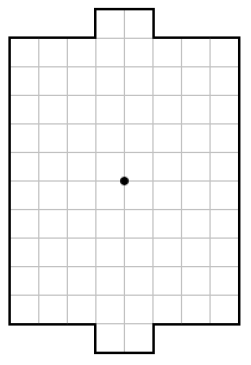
\includegraphics[width=0.2\textwidth]{board}
    \caption{Pusta plansza}
    
    \centering
    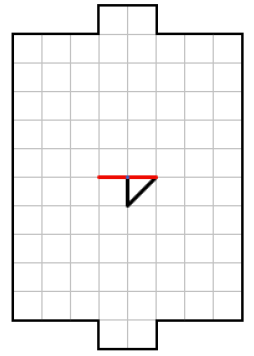
\includegraphics[width=0.2\textwidth]{odbicie}
    \caption{Odbicie (kolor czerwony)}
    
    \centering
    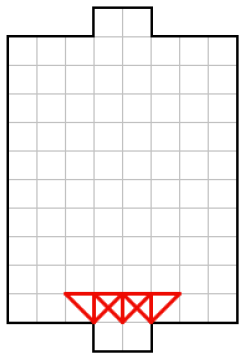
\includegraphics[width=0.2\textwidth]{zablokowanie}
    \caption{Zablokowanie bramki}
\end{wrapfigure}

Piłkarzyki na kartce to gra strategiczna, odbywającą się na prostokątnym boisku, rysowanym zazwyczaj na kartce w kratę.
Gracze na przemian wykonują ruchy polegające na przemieszczeniu piłki na sąsiednie pola, aż znajdzie się ona w jednej z bramek lub nie będzie możliwe wykonanie kolejnego ruchu.

Najczęściej stosowanym wymiarem planszy jest 8x10 kratek.
Przy krótszych bokach narysowane są dwie bramki o szerokości 2 kratek, w których gracze muszą umieścić piłkę.
Rozgrywka toczy się jedynie na przecięciach linii.
Środek planszy jest punktem startowym gry, do którego gracze dorysowują kolejne linie, oznaczające przemieszczenie piłki na sąsiednie pole. Każdy kolejny ruch zaczyna się w miejscu, w którym skończył się poprzedni, wzdłuż kratki lub po przekątnej. 

Ruchy nie mogą odbywać się po brzegu planszy ani wzdłuż odcinków, po których wcześniej piłka była już prowadzona.
Możliwe jest odbijanie się, które polega na wykonaniu przez gracza dodatkowego ruchu. Następuje ono gdy ruch zostanie zakończony w miejscu, w którym kończy się już linia narysowana przez jednego z graczy lub na brzegu boiska. 

Gra kończy się w momencie gdy piłka znajdzie się w jednej z bramek.
Wówczas gracz, do którego należy dana bramka, przegrywa. 
Gracz może również przegrać w wypadku gdy nie jest w stanie wykonać żadnego ruchu.
 
 
\chapter{Uczenie ze Wzmocnieniem}\label{r:rl}

\section{Wprowadzenie}

Uczenie ze wzmocnieniem (ang. Reinforcement Learning, RL) jest działem uczenia maszynowego, zajmującym się sekwencyjnym podejmowaniem decyzji. Na proces uczenia składa się agent oraz środowisko, z którym wchodzi on w interakcje. 

todo dopisać o tym że akcje wykonujemy krok po kroku w czasie. napisać czym jest epizod

Po każdej wykonanej akcji, agent obserwuje jaką nagrodę otrzymał. Jest to jedyny sposób w jaki może on oceniać jakość podjętych przez siebie decyzji. 
Zadaniem agenta jest wyuczenie się optymalnej polityki - funkcji która każdemu stanowi przyporządkowuje akcję, która maksymalizuje wartość oczekiwaną sumy wszystkich przyszłych nagród. 
Podczas procesu uczenia się, nigdy nie wskazujemy agentowi którą akcje powinien on wykonać, co stanowi główną różnice pomiędzy uczeniem ze wzmocnieniem a uczeniem nadzorowanym (ang. Supervised Learning). 

\section{Dyskretny Proces Markowa}

Dyskretny Proces Markowa składa się z:
\begin{itemize}
\item zbioru stanów w których może znaleźć się agent, $ s \in \mathcal{S} $,
\item rozkładu stanu początkowego $\mathcal{D}$ nad zbiorem $\mathcal{S}$,
\item zbioru akcji możliwych do podjęcia przez agenta, $ a \in \mathcal{A} $
\item nagrody otrzymywanej przez agenta za każdym razem, gdy ten wykona jakąś akcje, $ r_t \in \mathbb{R} $
\item prawdopodobieństwa przejścia między stanami
$$ p(s'|s, a) = \mathbb{P}(s_{t+1} = s' \mid s_t = s, a_t = a)$$
\item funkcji nagrody, $ R : S \times S \times A \rightarrow \mathbb{R} $
$$ R(s, a, s') = \mathbb{E}(r_{t+1} \mid s_t = s, a_t = a, s_{t+1} = s') $$
\item współczynnik dyskontującego wartości nagród otrzymywanych w przyszłości $ \gamma \in [0, 1] $
\end{itemize}

Funkcja nagrody oraz prawdopodobieństwo przejścia są najbardziej istotnymi elementami MDP i są zazwyczaj nieznane podczas rozwiązywania problemu uczenia ze wzmocnieniem.

\section{Polityka}

Polityka jest funkcją która każdemu stanowi przyporządkowuje akcję. Może być ona deterministyczna, $ \pi(s) $, bądź też stochastyczna, $ \pi(a \mid s) $, i wówczas stanowić rozkład prawdopodobieństwa wszystkich akcji dla ustalonego stanu. Metody uczenia ze wzmocnieniem określają w jaki sposób polityka jest modyfikowana na podstawie doświadczenia zbieranego przez agenta.

\section{Zakumulowana Nagroda}

Naszym celem jest znalezienie polityki, która będzie maksymalizować wartość oczekiwaną sumy nagród, które nasz agent otrzyma w przyszłości. Sumę nagród określmy mianem \emph{zakumulowanej nagrody}, $ G_t $, która zdefiniowana jest następująco:

$$ G_t = r_{t+1} + r_{t+2} + r_{t+3} + ... + r_{T-1} = r_{t+1} + G_{t+1} $$

gdzie $T$ jest końcem epizodu, a $t$ indeksem czasu.

Możemy również skorzystać z \emph{zdyskontowanej zakumulowanej nagrody}, która zdefiniowana jest następująco:

$$ G_t = r_{t+1} + \gamma r_{t+2} + \gamma^2 r_{t+3} + ... + \gamma^{T-1}r_{T} = 
\sum_{k=0}^{T-1} \gamma^k r_{t+k+1} $$

Szczególnie przydatna jest ona w przypadku nieograniczonych epizodów, wówczas:

$$ G_t = r_{t+1} + \gamma r_{t+2} + \gamma^2 r_{t+3} + ...  = 
\sum_{k=0}^{\infty} \gamma^k r_{t+k+1} $$

wtedy $ \gamma \in [0, 1) $.

\section{Funkcja Wartości}

Posiadając już politykę naszego agenta, możemy chcieć się dowiedzieć jaką nagrodę uzyska agent, który będzie jej przestrzegał. W tym celu definiujemy \emph{funkcję wartości stanu} (ang. Value Function), którą oznaczamy jako $ v_{\pi}(s) $ dla ustalonej polityki $ \pi $. Definiujemy ją jako:

$$ v_{\pi}(s) = \mathbb{E}_{\pi}[G_t \mid S_t = s] = \mathbb{E}_{\pi} \Bigg[ \sum_{k=0}^{\infty} \gamma^k R_{t+k+1} \bigg| S_t = s \Bigg] $$

gdzie $ \mathbb{E}_{\pi} $ jest wartością oczekiwaną przy założeniu że agent kieruje się polityką $\pi$, z kolei $t$ jest dowolnym punktem w czasie. 

Podobnie definiujemy wartość wybrania akcji $a$, gdy znajdujemy się w stanie $s$ oraz podążamy zgodnie z polityką $\pi$, oznaczaną jako $q_{\pi}(s, a)$. Jest ona wartością oczekiwaną z sytuacji w której rozpoczynamy w stanie $s$, wykonujemy akcję $a$, po czym wszystkie kolejne akcje wykonujemy zgodnie z polityką $\pi$. Funkcję tę nazywamy \emph{funkcją wartości akcji}.

$$ q_{\pi}(s, a) = \mathbb{E}_{\pi}[G_t \mid S_t = s, A_t = a] = \mathbb{E}_{\pi} \Bigg[ \sum_{k=0}^{\infty} \gamma^k R_{t+k+1} \bigg| S_t = s, A_t = a \Bigg] $$

\section{Optymalność polityki oraz funkcji wartości}

Podczas rozwiązywania problemu uczenia ze wzmocnieniem staramy się znaleźć politykę, której przestrzeganie przyniesie naszemu agentowi jak największą nagrodę. Będziemy mówić że polityka $\pi$ jest lepsza lub równa polityce $\pi'$, wtedy i tylko wtedy gdy oczekiwana nagroda dla niej jest większa lub równa niż dla $\pi'$ w każdym stanie należącym do przestrzeni stanów. Zawsze istnieje polityka, która jest lepsza lub równa od wszystkich innych i nazywamy ją \emph{optymalną polityką}. Może istnieć wiele różnych od siebie optymalnych polityk, jednak każdą z nich oznaczamy jako $\pi_{\ast}$. Dla wszystkich z nich funkcja wartości stanu jest taka sama i nazywamy ją \emph{optymalną funkcją wartości stanu}. Spełnia ona własność:

$$ v_{\ast}(s) = \max_{\pi} v_{\pi}(s) $$

dla każdego stanu $s \in \mathcal{S}$. Podobnie współdzielą one \emph{optymalną funkcję wartości akcji}, $q_{\ast}$, która spełnia:

$$ q_{\ast}(s, a) = \max_{\pi} q_{\pi}(s, a) $$

dla każdego stanu $s \in \mathcal{S}$ oraz akcji $a \in \mathcal{A}$.

Ponadto optymalną funkcję wartości stanu możemy zdefiniować odwołując się do funkcji wartości akcji w następujący sposób:

$$ v_{\ast}(s) = \max_{a \in \mathcal{A}} q_{\pi_{\ast}}(s) $$

Podstawową własnością, jaką spełniają funkcje wartości, jest \emph{równanie Bellmana}. Dla dowolnej polityki $\pi$ oraz stanu $s$ zachodzi:

\begin{align}
v_{\pi}(s) &= \mathbb{E}_{\pi}[G_t \mid S_t = s]  \nonumber \\
&= \mathbb{E}_{\pi}[r_{t+1} + \gamma G_{t+1} \mid S_t = s] \nonumber \\
&= \sum_a \pi(a \mid s) \sum_s' \sum_r p(s', r \mid s, a) \Big[r + \gamma \mathbb{E}_{\pi}[G_{t+1} \mid S_{t+1} = s' ]\Big] \nonumber \\
&= \sum_a \pi(a \mid s) \sum_{s', r} p(s', r \mid s, a) \Big[r + \gamma v_{\pi}(s') \Big]
\end{align}

Na podstawie własności optymalnych funkcji wartości oraz równania Bellmana możemy wyprowadzić \emph{równania optymalności Bellmana}, bez odwoływania się przy tym do żadnej polityki. Pierwsze z nich odnosi się do funkcji wartości stanu:

\begin{align}
v_{\ast}(s) &= \max_{a \in \mathcal{A}} q_{\pi_{\ast}}(s, a) \nonumber \\
&= \max_a \mathbb{E}_{\pi}[G_t \mid S_t = s, A_t = a]  \nonumber \\
&= \max_a \mathbb{E}_{\pi}[r_{t+1} + \gamma G_{t+1} \mid S_t = s, A_t = a] \nonumber \\
&= \max_a \mathbb{E}[r_{t+1} + \gamma v_{\pi_{\ast}}(S_{t+1}) \mid S_t = s, A_t = a] \nonumber \\
&= \max_a \sum_{s', r} p(s', r \mid s, a) \Big[r + \gamma v_{\ast}(s') \Big]
\end{align}

Natomiast drugie zdefiniowane jest dla funkcji wartości akcji:

\begin{align}
q_{\ast}(s, a) &= \mathbb{E}[r_{t+1} + \gamma \max_{a'} q_{\ast} (S_{t+1}, a') \mid S_t = s, A_t = a] \nonumber \\
&= \sum_{s', r} p(s', r \mid s, a) \Big[r + \gamma \max_{a'} q_{\ast} (s', a') \Big]
\end{align}


\section{Metody nie uwzględniające Modelu}



\subsection{Metody bazujące na Funkcji Wartości} 

\subsection{Metody bazujące na Polityce} 

\subsection{Metody Aktor-Krytyk}

\section{Podsumowanie}

\chapter{Głębokie Sieci Neuronowe}

\chapter{Głębokie Uczenie ze Wzmocnieniem}

\begin{thebibliography}{99}
\addcontentsline{toc}{chapter}{Bibliografia}

\bibitem[Bea65]{beaman} Juliusz Beaman, \textit{Morbidity of the Jolly
    function}, Mathematica Absurdica, 117 (1965) 338--9.

\bibitem[Blar16]{eb1} Elizjusz Blarbarucki, \textit{O pewnych
    aspektach pewnych aspektów}, Astrolog Polski, Zeszyt 16, Warszawa
  1916.

\bibitem[Fif00]{ffgg} Filigran Fifak, Gizbert Gryzogrzechotalski,
  \textit{O blabalii fetorycznej}, Materiały Konferencji Euroblabal
  2000.

\bibitem[Fif01]{ff-sr} Filigran Fifak, \textit{O fetorach
    $\sigma$-$\rho$}, Acta Fetorica, 2001.

\bibitem[Głomb04]{grglo} Gryzybór Głombaski, \textit{Parazytonikacja
    blabiczna fetorów --- nowa teoria wszystkiego}, Warszawa 1904.

\bibitem[Hopp96]{hopp} Claude Hopper, \textit{On some $\Pi$-hedral
    surfaces in quasi-quasi space}, Omnius University Press, 1996.

\bibitem[Leuk00]{leuk} Lechoslav Leukocyt, \textit{Oval mappings ab ovo},
  Materiały Białostockiej Konferencji Hodowców Drobiu, 2000.

\bibitem[Rozk93]{JR} Josip A.~Rozkosza, \textit{O pewnych własnościach
    pewnych funkcji}, Północnopomorski Dziennik Matematyczny 63491
  (1993).

\bibitem[Spy59]{spyrpt} Mrowclaw Spyrpt, \textit{A matrix is a matrix
    is a matrix}, Mat. Zburp., 91 (1959) 28--35.

\bibitem[Sri64]{srinis} Rajagopalachari Sriniswamiramanathan,
  \textit{Some expansions on the Flausgloten Theorem on locally
    congested lutches}, J. Math.  Soc., North Bombay, 13 (1964) 72--6.

\bibitem[Whi25]{russell} Alfred N. Whitehead, Bertrand Russell,
  \textit{Principia Mathematica}, Cambridge University Press, 1925.

\bibitem[Zen69]{heu} Zenon Zenon, \textit{Użyteczne heurystyki
    w~blabalizie}, Młody Technik, nr~11, 1969.

\end{thebibliography}

\end{document}


%%% Local Variables:
%%% mode: latex
%%% TeX-master: t
%%% coding: latin-2
%%% End:
